\newpage
\subsection{Declaring classes and attributes}
\texHeader
\hypertarget{static:classes tex}{}

% Discuss syntax in this section! (We removed it from Part I)
\begin{itemize}

\item[$\blacktriangleright$] Right click on the \texttt{LearningBoxLanguage} subfolder and create your first EClass model by going to ``New/EClass.'' Name it `Box'.

\vspace{0.5cm}

\item[$\blacktriangleright$] The class editor should automatically open. Currently, it's empty; Let's add the first two EAttributes of our program,
\texttt{name} and \texttt{stringRep}. Both are \texttt{EString} types (Fig.~\ref{fig:boxDeclaration}).

\vspace{0.5cm}

\begin{figure}[htbp]
	\centering
  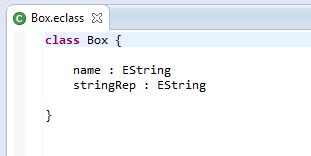
\includegraphics[width=0.4\textwidth]{eclipse_classBoxDeclaration}
	\caption{Newly created box class}
	\label{fig:boxDeclaration}
\end{figure} 

\item[$\blacktriangleright$] Create two more empty classes in your model the same way, \texttt{Partition} and \texttt{Card}.

\vspace{0.5cm}

\item[$\blacktriangleright$] In \texttt{Partition}, add two \texttt{EInt} datatypes, \texttt{index} and \texttt{partitionSize}.

\vspace{0.5cm}

\item[$\blacktriangleright$] In \texttt{Card}, create three \texttt{EString}s, \texttt{back}, \texttt{face} , and \texttt{partitionHistory}.

\vspace{0.5cm}

\item[$\blacktriangleright$] If you've done everything correctly, the key areas of your workspace should now resemble Fig.~\ref{fig:workspaceClassAttributes}.

\vspace{0.5cm}

\item[$\blacktriangleright$] Closing message; While some languages (such as Java) allow you to declare several small classes such as these in the same file,
when tooling with eMolfon, it's best to have them separated. The MOSL builder will not give you an error if you implement them this way, but none of your
program's dynamic actions will work. Don't worry - we'll explain this later in the handbook.

\newpage

\vspace*{3cm}

\begin{figure}[htbp]
	\centering
  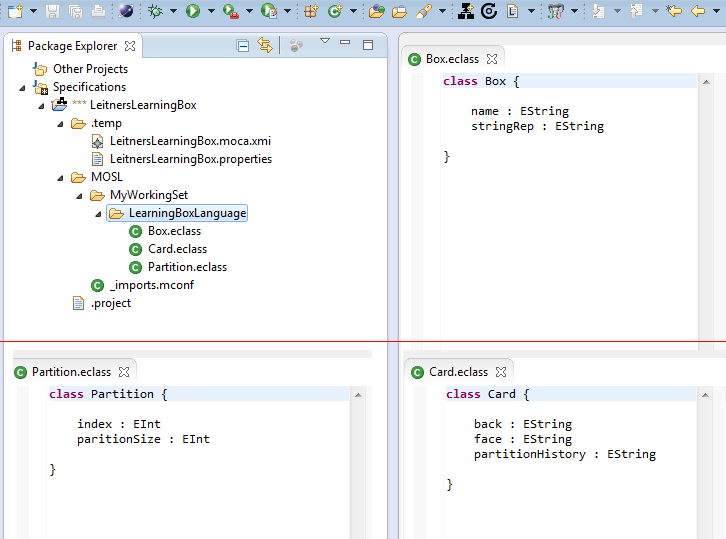
\includegraphics[width=1.0\textwidth]{eclipse_workspaceClassesAttributes}
	\caption{Declaration of classes and attributes}
	\label{fig:workspaceClassAttributes}
\end{figure} 

\fancyfoot[R]{$\triangleright$ \hyperlink{static:references splash}{Next}}

\end{itemize}
